\documentclass{article}
\usepackage{geometry}
\geometry{landscape}

\usepackage{tikz}
\usetikzlibrary{trees}

\begin{document}

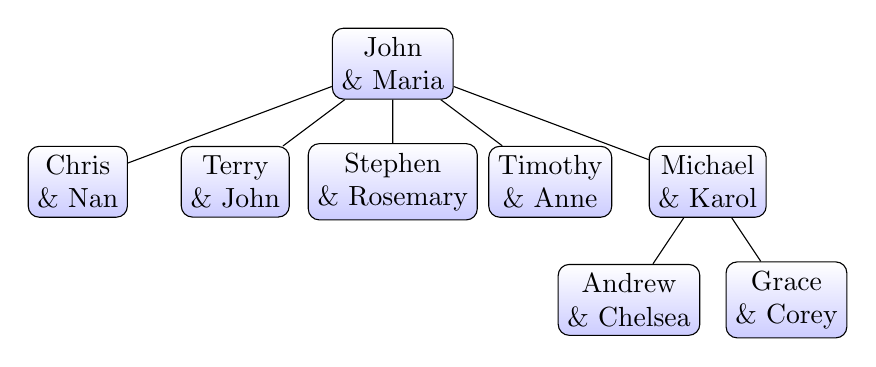
\begin{tikzpicture}[
  sibling distance=20mm, 
  level distance=15mm,
  every node/.style = {
    shape=rectangle, 
    rounded corners,
    draw, 
    align=center,
    top color=white, 
    bottom color=blue!20
  }
]

\node {John \\\& Maria}
    child { node {Chris \\\& Nan} }
    child { node {Terry \\\& John} }
    child { node {Stephen \\\& Rosemary} }
    child { node {Timothy \\\& Anne} }
    child { node {Michael \\\& Karol}
        child { node {Andrew \\\& Chelsea} }
        child { node {Grace \\\& Corey} }
    };

\end{tikzpicture}
\newpage

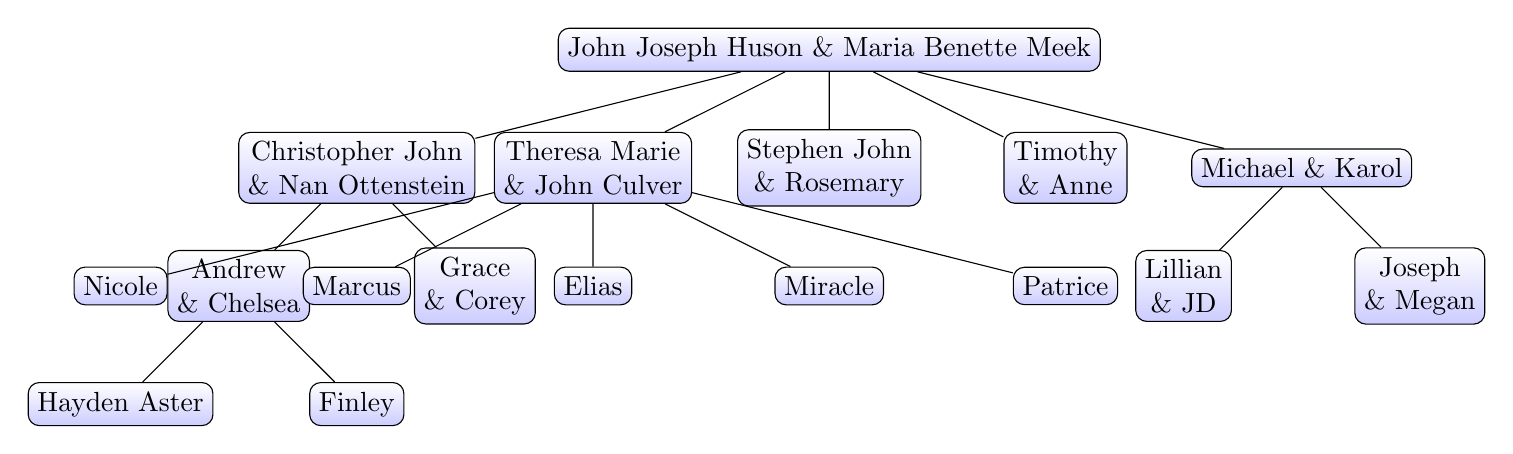
\begin{tikzpicture}[
    sibling distance=30mm, 
    level distance=15mm,
    every node/.style = {
      shape=rectangle, 
      rounded corners,
      draw, 
      align=center,
      top color=white, 
      bottom color=blue!20
    }
  ]
  
  \node {John Joseph Huson \& Maria Benette Meek}
      child { node {Christopher John \\\& Nan Ottenstein}
        child { node {Andrew \\\& Chelsea} 
            child { node {Hayden Aster} }
            child { node {Finley} }        }
        child { node {Grace \\\& Corey} } }
      child { node {Theresa Marie \\\& John Culver} 
        child { node {Nicole} }
        child { node {Marcus} }
        child { node {Elias} }
        child { node {Miracle} }     
        child { node {Patrice} }
        }
      child { node {Stephen John \\\& Rosemary} }
      child { node {Timothy \\\& Anne} }
      child { node {Michael \& Karol}
        child { node {Lillian \\\& JD} }
        child { node {Joseph \\\& Megan} }
      };
  
  \end{tikzpicture}

\end{document}
